
\documentclass{beamer}
\usetheme{Rochester}
\usepackage{fontspec}
\usepackage{xunicode}
\usepackage{xltxtra}
\usepackage{xecyr}
\usepackage{hyperref}
\setmainfont[Mapping=tex-text]{DejaVu Serif}
\setsansfont[Mapping=tex-text]{DejaVu Sans}
\setmonofont[Mapping=tex-text]{DejaVu Sans Mono}
\usepackage{polyglossia}
\setdefaultlanguage{russian}
\usepackage{graphicx}
\usepackage{listings}
\usepackage{multirow}
\usepackage{enumitem}
\usepackage{subcaption}
\usepackage{epsfig}            
\usepackage{cite}
\usepackage{tikz}
\usepackage{pgfplots}

\lstdefinestyle{mycode}{
  belowcaptionskip=1\baselineskip,
  breaklines=true,
  xleftmargin=\parindent,
  showstringspaces=false,
  basicstyle=\footnotesize\ttfamily,
  keywordstyle=\bfseries,
  commentstyle=\itshape\color{gray!40!black},
  stringstyle=\color{red},
  numbers=left,
  numbersep=5pt,
  numberstyle=\tiny\color{gray},
}
\lstset{escapechar=@,style=mycode}

\usepackage{enumitem}
\setlist[itemize,1]{label={\fontfamily{cmr}\fontencoding{T1}\selectfont\textbullet}}
\setbeamertemplate{enumerate items}[ball]

\begin{document}

\title[Бакалаврская работа]{Рандомизированный алгоритм при обработке данных ультразвуковых исследований}

\author[Иван Сенин]{
    \begin{flushright}
    И.\,И. Сенин \\
    {\footnotesize\textcolor{gray}\raggedleft{группа 444\\Научный руководитель:\\д.\,ф.-м.\,н., профессор О.\,Н. Граничин}}
    \end{flushright}
}

\institute{СПбГУ}
\date{2016}


\frame{\titlepage}

% --------------------------------------------------------------------------------
\begin{frame}
\frametitle{Введение}
\framesubtitle{Ультразвуковая томография}

\begin{columns}
	\begin{column}{0.4\textwidth}
		\begin{figure}[h]
    		\centering
    		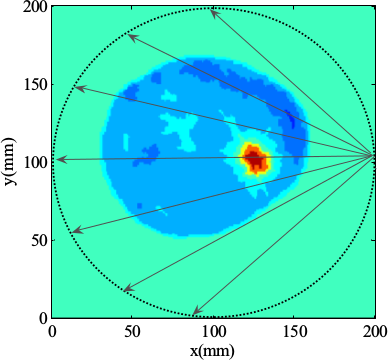
\includegraphics[width=\textwidth]{pics/tomo_scheme.png}
    		\caption{\small Схематичное изображение томографа}
    		\label{fig:pic1}
		\end{figure}
    \end{column}
    \begin{column}{0.55\textwidth}
		\begin{figure}[h]
      		\centering
      		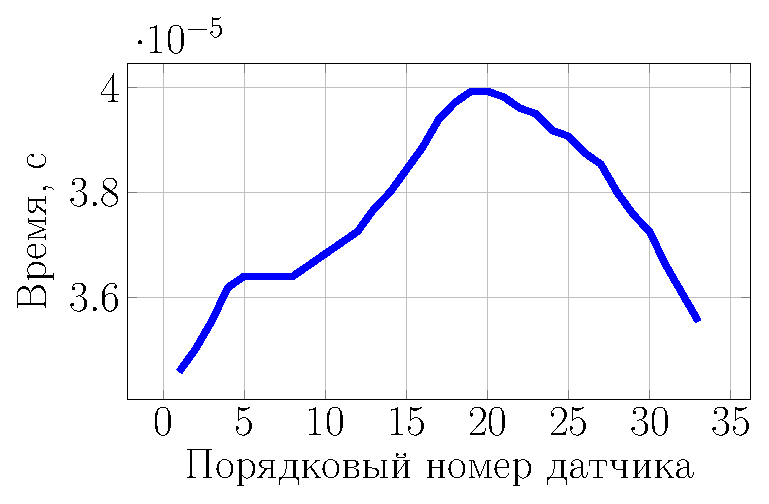
\includegraphics[width=\textwidth]{pics_eps/arrivals.eps}
      		\caption{Время прибытия сигнала на противоположные датчики}
      		\label{fig:pic2}
		\end{figure}
    \end{column}
\end{columns}


\end{frame}

% --------------------------------------------------------------------------------
\begin{frame}
\frametitle{Введение}
\framesubtitle{Метод реконструкции}
\begin{itemize}
	\item Решение обратной задачи: метод LASSO
\end{itemize}
$$ \min_F  \sqrt{\displaystyle\sum_{i=1}^{M} (|\displaystyle\sum_{j=1}^N A_{i,j}F_j - Y_i |^2)} + \lambda \displaystyle\sum_{i=1}^N \displaystyle\sum_{j=1}^N| \Psi_{i,j} F_j| $$
$A$ --- матрица расстояний, пройденных звуковой волной\\
$F$ --- искомый вектор распределения скорости\\
$Y$ --- время прибытия сигнала\\
$\Psi$ --- вейвлет-преобразование\\
$\lambda$ --- весовой коэффициент\\
$N$ --- разрешение изображения \\
$M$ --- количество измерений\\
\end{frame}

% --------------------------------------------------------------------------------
\begin{frame}
\frametitle{Введение}
\framesubtitle{Пример устройства}
Системные характеристики\footnote{\tiny The SoftVue scanner\\\textit{Roy,Oliver, et al.} ``Breast imaging using ultrasound tomography: From clinical requirements to system design'' // Ultrasonics Symposium (IUS), 2013 IEEE International}:\\\small
2$\times$ Intel Xeon E5620, 192 ГБ ОЗУ,\\
4$\times$ (Intel Xeon E5620, 96 ГБ ОЗУ, 2x NVidia Tesla M2070)
\begin{table}[h]
\centering
\caption{\small Объем исходных данных на 1 срез [ГБ]}
\begin{tabular}{ c || c | c | c }
    \hline
    \multirow{2}{*}{Частота дискретизации (МГц)} & \multicolumn{3}{c}{Число датчиков}  \\ %\cline{2-4}
    & 256 & 512 & 1024 \\
    \hline
    10 & 0.21 & 0.86 & 3.44 \\
    14 & 0.30 & 1.20 & 4.81 \\
    \hline
\end{tabular}
\end{table}
\normalsize

Время на обработку одного среза: 20 секунд\\
Количество срезов: 70\\
Общее время на обработку данных: 23.3 минуты\\

\end{frame}

% --------------------------------------------------------------------------------
\begin{frame}
\frametitle{Постановка задачи}
%\framesubtitle{Цели работы}
\begin{itemize}
\item Исследовать применимость техники ``опознание со сжатием'' в задаче ультразвуковой томографии
\item Разработать рандомизированный алгоритм для сбора и обработки данных ультразвуковой томографии
\item Провести эксперименты на программной симуляции
\item Реализовать вычислительное ядро алгоритма на языке Hascol
\end{itemize}

\end{frame}

% --------------------------------------------------------------------------------
\begin{frame}
\frametitle{Решение}
\framesubtitle{Достаточное количество измерений}
$$m \approx 4s\log{\frac{N}{s}}$$
\begin{table}[h]
	\centering
	\caption{Достаточное количество измерений}
	\begin{tabular}{| c | c | c | c |}
    	\hline
		$M$ & 64$\times$64 & 512$\times$512 & 1024$\times$1024 \\
    	\hline
    	$m$ & 1705 & 3718 & 4389 \\
    	\hline
	\end{tabular}
\end{table}

\small
$N$ --- разрешение изображения\\
$s$ --- характеристика разреженности сигнала\\
$m$ --- достаточное для CS количество измерений\\
$M$ --- полное количество измерений ($M\approx N$)
\normalsize

\end{frame}

% --------------------------------------------------------------------------------
\begin{frame}
\frametitle{Решение}
\framesubtitle{Достаточное количество измерений}

\begin{figure}[h]
	\centering
	\begin{tikzpicture}
         \begin{axis}[
         width=0.9\textwidth,
         height=3cm,
         view={0}{90},
         grid=major, 
         scale only axis,
         xtick={0, 500, 1000, 1500, 2000},
         xlabel={Количество датчиков в устройстве},
         ylabel={$m / M \times 100\% $}]
         \addplot+[line width=2pt, mark=none,shader=interp] table [x=x, y=y, col sep=comma, mark=none] {csv/percents_estimation.csv};
         \end{axis}
     \end{tikzpicture}
	\caption{Количество данных относительно исходного алгоритма в [\%]}
\end{figure}

\end{frame}


% --------------------------------------------------------------------------------
\begin{frame}
\frametitle{Решение}
\framesubtitle{Поиск вектора скоростей в разреженном представлении}
\begin{itemize}
	\item Решение обратной задачи: метод LASSO
\end{itemize}
$$ \min_X  \sqrt{\displaystyle\sum_{i=1}^{M} (\displaystyle\sum_{j=1}^N | \Phi_{i,j}X_j - \hat{A}Y_j |^2)} + \lambda \displaystyle\sum_{i=1}^N |X_i| $$
\small
$\hat{A}$ --- рандомизированная матрица измерений\\
$X$ --- искомый вектор в разреженном представлении\\
$\Phi=\hat{A}\cdot A\Psi$\\
\hfill\\
Используемые библиотеки MATLAB:
\begin{itemize}
\item Toolbox Fast Marching
\item Rice Wavelet Tools
\end{itemize}

\end{frame}

% --------------------------------------------------------------------------------
\begin{frame}
\frametitle{Решение}
\framesubtitle{Результаты эксперимента}
\begin{table}\small
\caption{\small Качество реконструкции снимка}
\centering
\begin{tabular}{| l | c | c | }
    \hline
    Матрица измерений & SNR, dB & RMSE, м/с \\
    \hline
    Базовая матрица & $\mathbf{23.89 \pm 0.06}$ & $\mathbf{181.89 \pm 1.30}$ \\
    Равновероятный отсев & $23.84 \pm 0.06$ & $183.06 \pm 1.34$ \\
    Отсев проекций & $23.77 \pm 0.07$ & $184.59 \pm 1.48$ \\
    Точечный выбор данных & $23.80 \pm 0.04$ & $184.15 \pm 0.85$ \\
    \hline
    Исходный алгоритм & 23.63 & 183.36 \\
    \hline
\end{tabular}
\end{table}

\vspace*{-3mm}
\begin{figure}[!tbp]
    \centering
    \begin{minipage}[b]{0.49\textwidth}
    	\raggedleft
        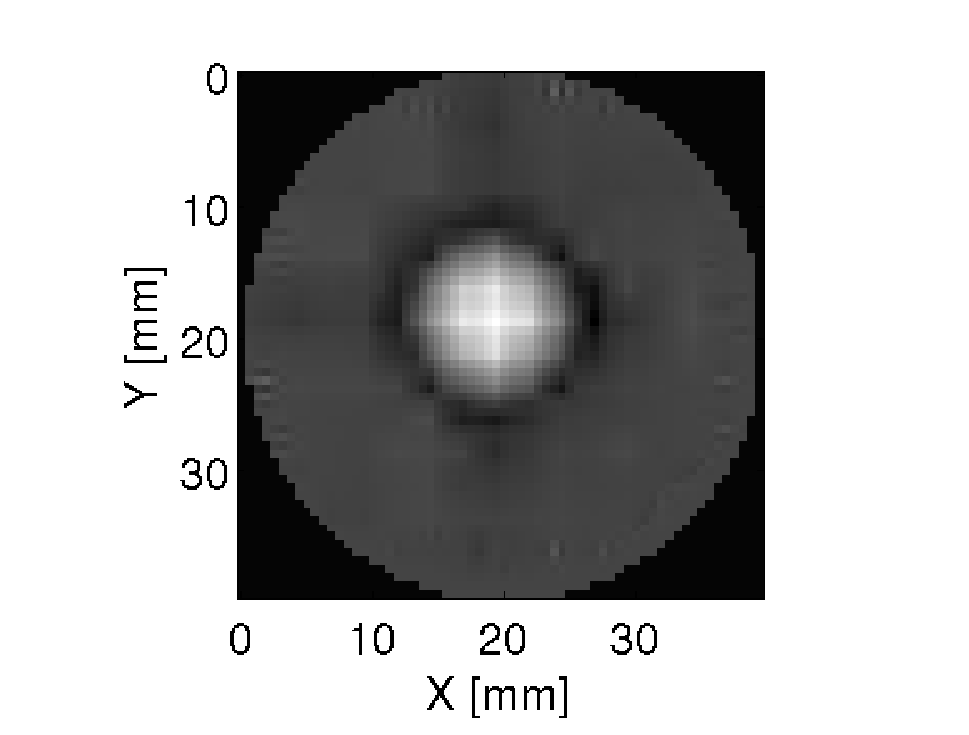
\includegraphics[scale=0.22]{pics_eps/slice_base_grad.eps}
    \end{minipage}
    \hfill
    \begin{minipage}[b]{0.49\textwidth}
        \raggedright
        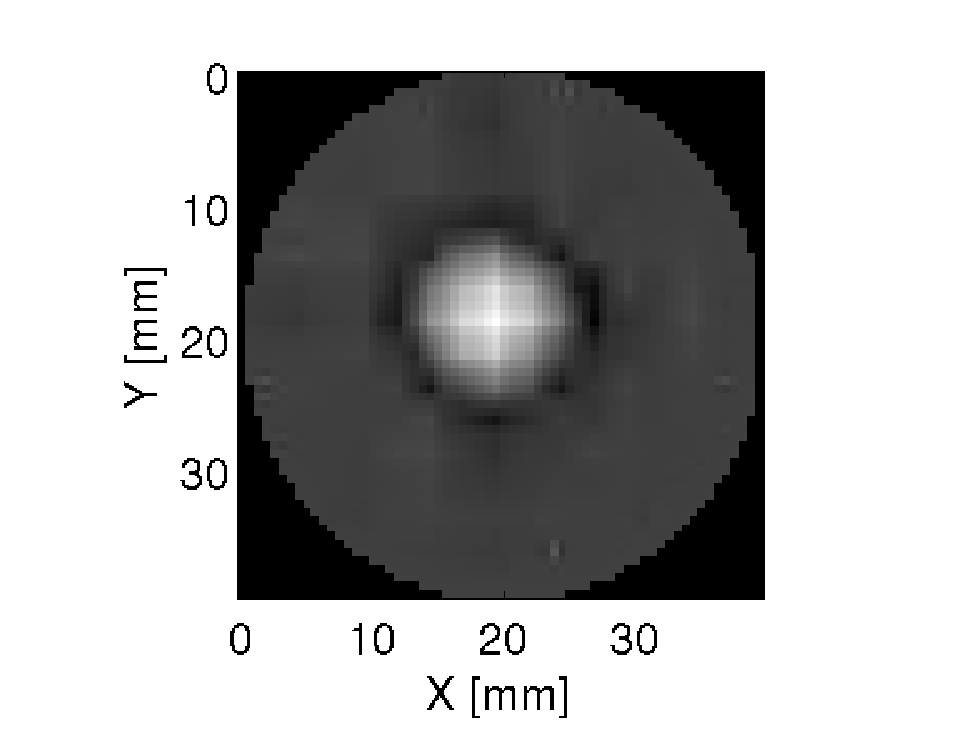
\includegraphics[scale=0.22]{pics_eps/slice_cs_grad.eps}
    \end{minipage}
    \caption{\footnotesize Результаты реконструкции исходного алгоритма (слева) и Compressive Sensing (справа).}
\end{figure}

\end{frame}


% --------------------------------------------------------------------------------
\begin{frame}
\frametitle{Решение}
\framesubtitle{Результаты эксперимента}
\begin{figure}[h]
\centering
    \begin{tikzpicture}
        \begin{axis}[
        width=.8\textwidth,
        height=3.5cm,
        view={0}{90},
        grid=major, 
        scale only axis,
        %xtick={0, 400, 800, 1200, 1600},
        xlabel={Процент использованных данных},
        ylabel={Ошибка (RMSE), м/с}]
        \addplot+[line width=2pt,mark=none] table [x=x, y=y, col sep=comma, mark=none] {csv/rmse_seq.csv};
        \addplot+[line width=2pt,dashed, mark=none] table [x=x, y=original, col sep=comma, mark=none] {csv/rmse_seq.csv}; %line width=3pt
        \legend{CS-i.i.d., Legacy}
        \end{axis}
    \end{tikzpicture}
    %\caption{Зависимость ошибки реконструкции снимка от объема использованных данных при использовании Compressive Sensing с матрицей измерений с равновероятным отсевом(CS-i.i.d.). Для сравнения показан результат исходного алгоритма, использующий полный объем данных (Legacy)}
    \caption{\small Зависимость ошибки реконструкции от объема использованных данных. Для сравнения показан результат исходного алгоритма (100\% данных) "Legacy"}
\end{figure}

\end{frame}



% --------------------------------------------------------------------------------
\begin{frame}
\frametitle{Результаты}
\begin{itemize}\small
\item Спроектирован и реализован на языке MATLAB алгоритм, использующий технику ``Опознание со сжатием'' для задачи обработки данных ультразвуковой томографии
\item Технология показала эффективность: сокращение необходимого объема данных до 68\% на маломасштабной модели симуляции
\item Алгоритм используется в совместном исследовании ультразвуковой томографии кафедрой биомедицинской инженерии университета ``Huazhong University of Science and Technology''
\item Результаты опубликованы в журнале ``Стохастическая оптимизация в информатике''
\item{[WIP]} Вычислительное ядро алгоритма реализовано на языке Hascol
\end{itemize}


\end{frame}

\end{document}


